\subsection{Neural Language Models (NLMs)}
The idea underlying NLMs is to project words from a corpus onto a continuous space and then apply a probability estimator that operates on that space. Initially, feedforward architecture was utilised in neural networks for language modelling~\cite{advancesnlm}.

Feedforward neural networks(FFNN) are used to train a statistical model of the distribution of word sequences. Feedforward NN LMs have the disadvantage of not having longer distance dependencies since they are essentially N-gram language models~\cite{advancesnlm}. However, unlike N-grams, Feedforward NN LMs do not require a lower order ((N-1)-gram) because the probabilities are interpolated for each feasible sequence of length N-1~\cite{largenlm}.

\subsubsection{Convoluted Neural Networks (CNNs)}
Convolutional neural networks (CNNs) apply a layer type known as a convolutional layer, which may extract features by combining a learnable filter (also called kernel)~\cite{cnn}. CNNs use hundreds of kernels (convolutional filters), each of which extracts a specific pattern of n-gram from the language. 
A new feature is produced by applying these convolutional operations to a window of words. Following that is max-over-time-pooling, which selects only the most essential feature (the feature with the highest value) for each feature map~\cite{sentencecnn, cnnclass}

CNNs are commonly used in computer vision and image processing.
Additionally, CNNs were also used for a variety of NLP tasks~\cite{object}. However, CNNs did not see much use in more advanced NLP applications such as prediction (Language modeling).

\subsubsection{Recurrent Neural Networks (RNNs)}
RNNs are designed to process sequences. The same algorithm is applied to each token in a sequence, and each step is dependent on the token and result before it. They have a hidden state, often known as a memory, that captures information about a sequence of previous inputs~\cite{Sherstinsky_2020}. The current input token and previous memory are used to update current memory. RNNs are fed sequentially with data from the whole corpus during training. The result is a probability distribution of upcoming words given the context (hidden state) and preceding word~\cite{Mikolov-lda}. RNNs are highly suited for language modelling and many other NLP applications due to the inherent sequential nature of language. The ability to capture unbounded context is made possible by RNNs (long distance dependencies) RNNs can process contexts of any length, which gives an advantage over FFNNs for language modelling~\cite{rnntrends}.

Slow training time was a drawback of this architecture, but this was resolved by using truncated back-propagation through time (truncated BPTT)~\cite{rnn}, an extension of back-propagation for RNNs in which an approximative gradient is computed at each word by using a fixed number of predecessor words.  As a result, the training context length is limited. The RNN's ability to retain long-term knowledge is increased by the addition of a feature layer that uses a context vector computed on sentence history using Latent Dirichlet Allocation (LDA). This feature layer represents topic information and is connected to both the hidden layer and the output layer~\cite{mikolov-rnn}.

\subsubsection{Long Short-Term Memory (LSTMs)}
LSTM networks~\cite{lstm} are a modified version of RNNs. There are three gates in an LSTM cell: an input gate, an output gate, and a forget gate. These gates determine whether to delete the memory or move data forward. The forget gate permits the error to back propagate an infinite number of time steps. These three gates are combined to compute the hidden state. The exploding/vanishing gradient problem is avoided by LSTM models, allowing LMs to simulate longer-distance dependencies.

The Encoder-Decoder RNN is made for sequence-to-sequence prediction, which involves taking a real-valued sequence and producing a prediction for another real-valued sequence. Machine translation is an example of a sequence to sequence prediction application. The fixed length intermediate representation has been demonstrated to be a performance bottleneck for encoder-decoder models, This may occur if exceptionally long sentences must be mapped into a fixed-length representation; performance degrades as sentence length rises~\cite{encoder}.

The attention mechanism is aimed at improving performance. It maps the words in the input sequence into words, which are then sent to the decoder, as opposed to mapping the entire input sequence into a fixed-length vector. As a result, only a select few (the most suitable) vectors are selected, avoiding the need to compress arbitrary long words into a fixed-length vector. The decoder intuitively focuses on specific segments of the input stream (hence the name Attention Mechanism). Self attention is an extension of attention in which relationships between sequence positions are computed to create a representation of the sequence~\cite{attention}.

\subsubsection{Transformer Models}
The transformer architecture is built using stacked self-attention mechanisms. This is done in an effort to prevent recurrence, as the training of RNNs can not be parallelized. There are six levels in both the encoder and the decoder~\cite{attention}. A FFNN and a self-attention mechanism (looking both at previous and future tokens) are the two components found in each encoder layer. The decoder contains an additional attention mechanism that enables it to pay attention to specific encoder segments, in contrast to the encoder layer. 
In a machine translation test, it was demonstrated that the transformer design outperformed several RNN and CNN based models~\cite{attention}. Figure~\ref{fig:transformer} shows the architecture of a transformer.

\begin{figure}[hbt!]
    \centering
    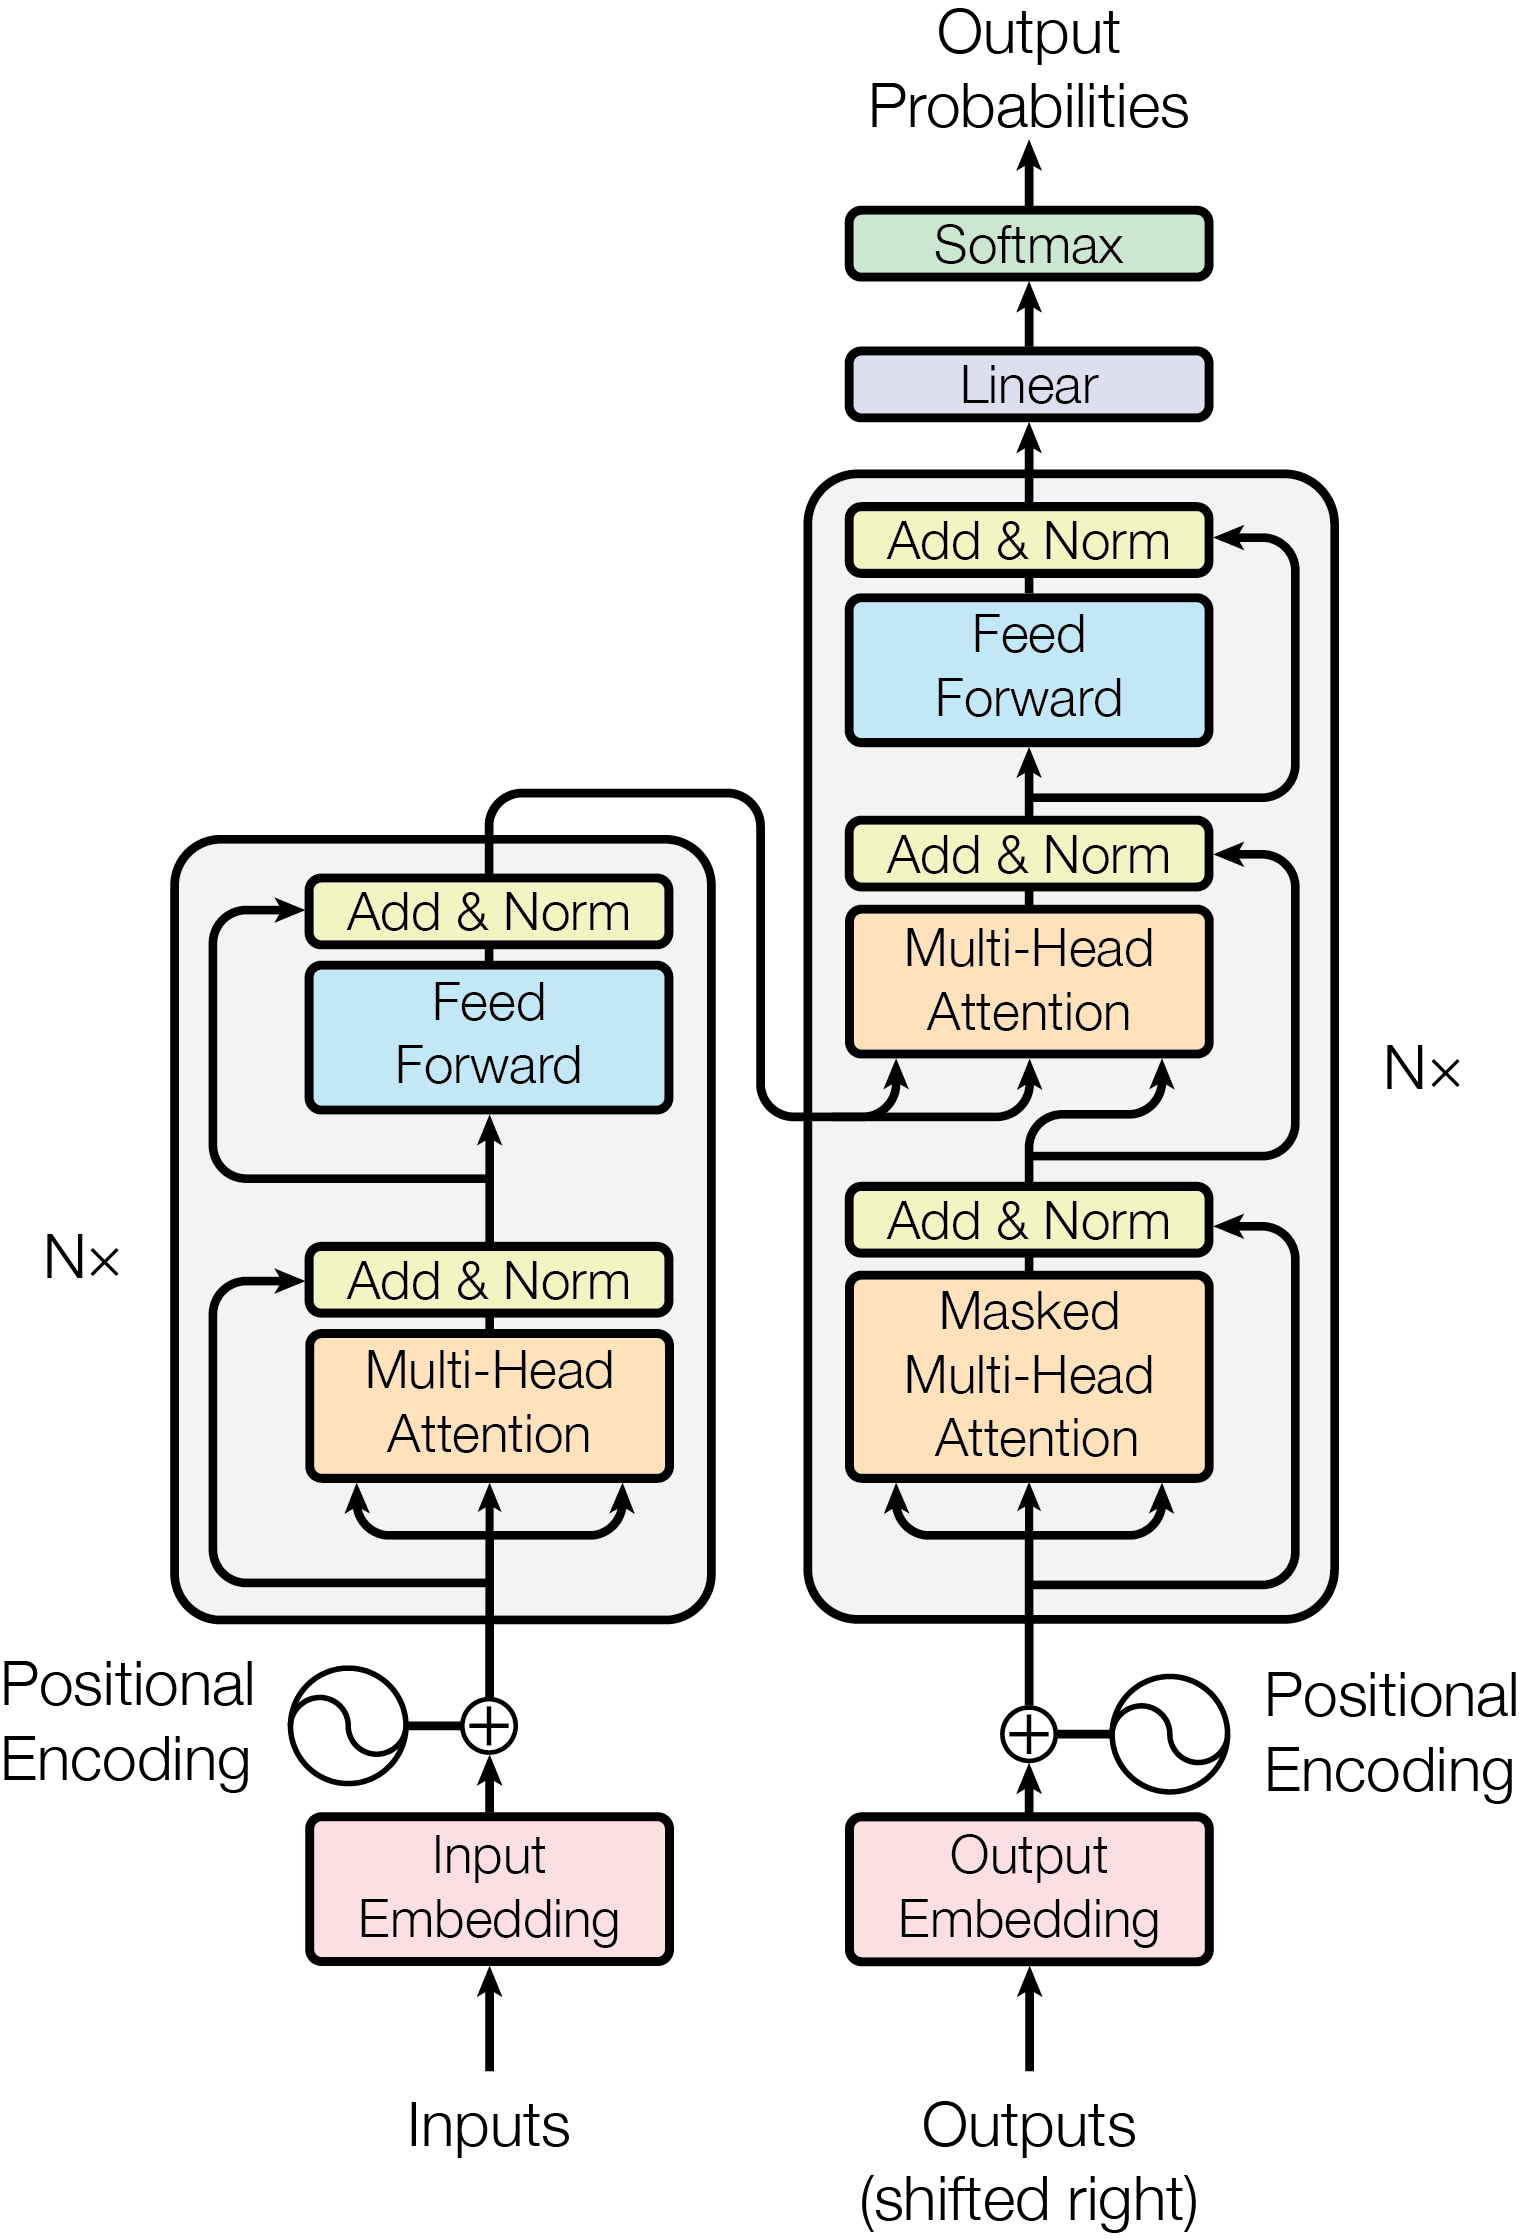
\includegraphics[width=.4\linewidth]{Figures/transformer.png}
    \caption{Transformer Architecture~\cite{attention}}
    \label{fig:transformer}
\end{figure}

\subsubsection{Contextualized Word Representations}
The encoding of words as fixed-length vectors allowed for the use of Deep Learning in NLP. The need that all word senses have the same representation presented a challenge. Context-sensitive contextualised word representations were presented by LMs such BERT~\cite{bert}, ELMo~\cite{elmo} and GPT-3~\cite{Gpt3}. BERT has a variant for general-purpose representations that support downstream applications such as natural language code-search, code documentation generation called CodeBERT~\cite{codebert}. This implies that representations of the same word vary depending on the context. Metrics in numerous NLP tasks have significantly improved because to these new word representations~\cite{contextual}. 